	%%%%%%%%%%%%%%%%%%%%%%%%%%%%%%%%%%%%%%%%%
% Beamer Presentation
% LaTeX Template
% Version 1.0 (10/11/12)
%
% This template has been downloaded from:
% http://www.LaTeXTemplates.com
%
% License:
% CC BY-NC-SA 3.0 (http://creativecommons.org/licenses/by-nc-sa/3.0/)
%
%%%%%%%%%%%%%%%%%%%%%%%%%%%%%%%%%%%%%%%%%

%----------------------------------------------------------------------------------------
%	PACKAGES AND THEMES
%----------------------------------------------------------------------------------------

\documentclass[handout]{beamer}

\mode<presentation> {

% The Beamer class comes with a number of default slide themes
% which change the colors and layouts of slides. Below this is a list
% of all the themes, uncomment each in turn to see what they look like.

%\usetheme{default}
%\usetheme{AnnArbor}
%\usetheme{Antibes}
%\usetheme{Bergen}
%\usetheme{Berkeley}
%\usetheme{Berlin}
%\usetheme{Boadilla}
%\usetheme{CambridgeUS}
%\usetheme{Copenhagen}
%\usetheme{Darmstadt}
%\usetheme{Dresden}
%\usetheme{Frankfurt}
%\usetheme{Goettingen}
%\usetheme{Hannover}
%\usetheme{Ilmenau}
%\usetheme{JuanLesPins}
%\usetheme{Luebeck}
\usetheme{Madrid}
%\usetheme{Malmoe}
%\usetheme{Marburg}
%\usetheme{Montpellier}
%\usetheme{PaloAlto}
%\usetheme{Pittsburgh}
%\usetheme{Rochester}
%\usetheme{Singapore}
%\usetheme{Szeged}
%\usetheme{Warsaw}

% As well as themes, the Beamer class has a number of color themes
% for any slide theme. Uncomment each of these in turn to see how it
% changes the colors of your current slide theme.

%\usecolortheme{albatross}
\usecolortheme{beaver}
%\usecolortheme{beetle}
%\usecolortheme{crane}
%\usecolortheme{dolphin}
%\usecolortheme{dove}
%\usecolortheme{fly}
%\usecolortheme{lily}
%\usecolortheme{orchid}
%\usecolortheme{rose}
%\usecolortheme{seagull}
%\usecolortheme{seahorse}
%\usecolortheme{whale}
%\usecolortheme{wolverine}

%\setbeamertemplate{footline} % To remove the footer line in all slides uncomment this line
%\setbeamertemplate{footline}[page number] % To replace the footer line in all slides with a simple slide count uncomment this line

%\setbeamertemplate{navigation symbols}{} % To remove the navigation symbols from the bottom of all slides uncomment this line
}

\usepackage{graphicx} % Allows including images
\usepackage{booktabs} % Allows the use of \toprule, \midrule and \bottomrule in tables
%\usepackage[T1]{fontenc}
\usepackage[utf8]{inputenc}
\usepackage{color}



\usepackage{listings}
\lstset{language=C}


%----------------------------------------------------------------------------------------
%	TITLE PAGE
%----------------------------------------------------------------------------------------

\title[Projet Minix]{Projet Minix - Défragmentation} % The short title appears at the bottom of every slide, the full title is only on the title page

\author[Colmonts - Van Ouytsel] {Julien Colmonts - Vincent Van Ouytsel} % Your name
\institute[UCL] % Your institution as it will appear on the bottom of every slide, may be shorthand to save space
{
Université Catholique de Louvain \\ % Your institution for the title page
\medskip

}
\date{\today} % Date, can be changed to a custom date

\begin{document}

\begin{frame}
\titlepage % Print the title page as the first slide
\end{frame}

%----------------------------------------------------------------------------------------
%	PRESENTATION SLIDES
%----------------------------------------------------------------------------------------

%------------------------------------------------
\section{Présentation de l'architecture} % Sections can be created in order to organize your presentation into discrete blocks, all sections and subsections are automatically printed in the table of contents as an overview of the talk
%------------------------------------------------

\begin{frame}
\frametitle{Présentation de l'architecture}
\begin{figure}
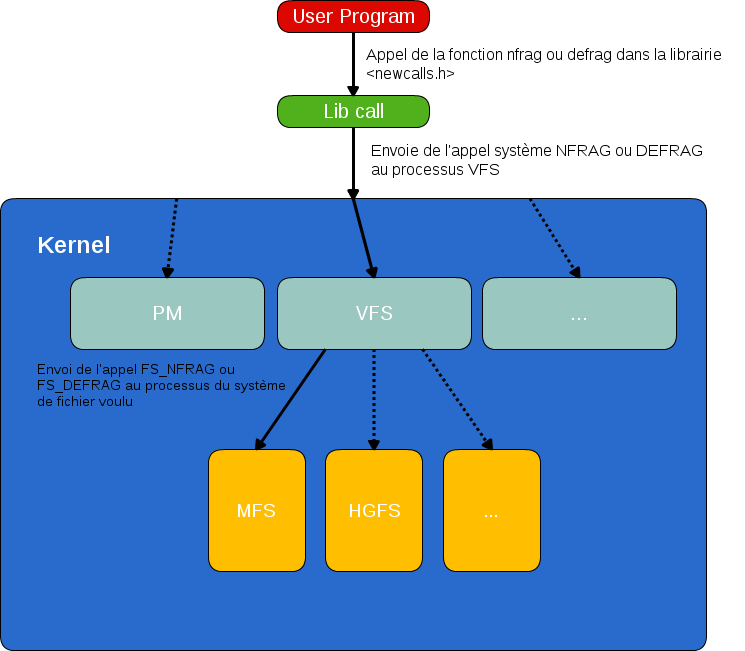
\includegraphics[scale=0.3]{schemas/archigen.png}
\end{figure}
\end{frame}

%------------------------------------------------

\begin{frame}
\frametitle{Les fichiers modifiés}
\begin{itemize}
\item \textsc{/src/include/minix/callnr.h} : ajout des constantes pour les deux nouveaux appels systèmes
\item \textsc{/src/servers/vfs/table.c} : introduction des noms de fonctions liées aux deux appels
\item \textsc{/src/servers/vfs/proto.h} : déclaration des fonctions, prototypes
\item \textsc{/src/servers/vfs/frag.c} : implémentation des fonctions
\item \textsc{/src/servers/vfs/request.c} : ajout des fonctions permettant d'effectuer les appels systèmes NFRAG et DEFRAG sur un système de fichiers MFS
\end{itemize}
\end{frame}

%------------------------------------------------

\begin{frame}[fragile]
\frametitle{Implémentation VFS}
\begin{block}{L'implémentation de l'appel système effectue les vérifications suivantes avant de poursuivre l'appel dans MFS}
\begin{lstlisting} 
if(fetch_name(m_in.name1,m_in.name1_length,M1)!=OK)
	    	return err_code; 
vn=eat_path(PATH_NOFLAGS,fp); 
if(vn == NULL) return err_code; 
if((vn->v_mode & I_TYPE) != I_REGULAR){
	put_vnode(vn);
	return EPERM; 
}
if (vp->v_ref_count != 1) return(EBUSY);
\end{lstlisting}
\end{block}
\end{frame}

%------------------------------------------------

\begin{frame}
\frametitle{Dans MFS}
\begin{block} {Appel système}
\begin{itemize}
\item Ajout des constantes d'appel
\item Transfert de données via le message sortant
\end{itemize}
\end{block}
\begin{block}{Comptage du nombre de fragments}
\begin{itemize}
\item Itération zone par zone
\end{itemize}
\end{block}
\end{frame}

%------------------------------------------------

\begin{frame}
\frametitle{Dans MFS}
\begin{block} {Stratégie de défragmentation}
\begin{itemize}
\item Comptage du nombre de fragments
\item Recherche d'une suite de zones libres suffisamment grande dans la \textsc{Zone Map}
\item Déplacement des données bloc par bloc dans la zone trouvée
\item Mise à jour des bitmaps
\end{itemize}
\end{block}
\end{frame}
%------------------------------------------------

\begin{frame}
\frametitle{Stratégie de test}
\begin{columns}[c]
\column{.4\textwidth}
\begin{itemize}
\item Création d'une partition
\item Montage
\item Création d'un fichier fragmenté
\item Tests de l'appel système
\end{itemize}
\column{.6\textwidth}
\begin{figure}
\includegraphics[scale=0.25]{schemas/test.png}
\end{figure}
\end{columns}
\end{frame}


%------------------------------------------------

\begin{frame}
\frametitle{Notre solution}
\begin{block}{Avantages}
\begin{itemize}
\item Respect des conventions de programmation dans \textsc{Minix}
\item Ajout de peu de fonctions dans le noyau, utilisation de fonctions déjà présentes
\item Tests passés avec succès
\end{itemize}
\end{block}
\begin{block}{Inconvénients}
\begin{itemize}
\item Le processus MFS ne doit traiter qu'un message à la fois
\item La comptage des fragments ne prend pas en compte les blocs indirects
\item La stratégie de défragmentation peut être améliorée (réduire le nombre de fragments sans atteindre 1, utiliser les zones occupées par le fichier à défragmenter, stratégie de défragmentation pour un système de fichiers complet,...)
\end{itemize}
\end{block}
\end{frame}

%------------------------------------------------




%\begin{frame}
%\frametitle{Blocks of Highlighted Text}
%\begin{block}{Block 1}
%Lorem ipsum dolor sit amet, consectetur adipiscing elit. Integer lectus nisl, ultricies in feugiat rutrum, porttitor sit amet augue. Aliquam ut tortor mauris. Sed volutpat ante purus, quis accumsan dolor.
%\end{block}
%
%\begin{block}{Block 2}
%Pellentesque sed tellus purus. Class aptent taciti sociosqu ad litora torquent per conubia nostra, per inceptos himenaeos. Vestibulum quis magna at risus dictum tempor eu vitae velit.
%\end{block}
%
%\begin{block}{Block 3}
%Suspendisse tincidunt sagittis gravida. Curabitur condimentum, enim sed venenatis rutrum, ipsum neque consectetur orci, sed blandit justo nisi ac lacus.
%\end{block}
%\end{frame}
%
%%------------------------------------------------
%
%\begin{frame}
%\frametitle{Multiple Columns}
%\begin{columns}[c] % The "c" option specifies centered vertical alignment while the "t" option is used for top vertical alignment
%
%\column{.45\textwidth} % Left column and width
%\textbf{Heading}
%\begin{enumerate}
%\item Statement
%\item Explanation
%\item Example
%\end{enumerate}
%
%\column{.5\textwidth} % Right column and width
%Lorem ipsum dolor sit amet, consectetur adipiscing elit. Integer lectus nisl, ultricies in feugiat rutrum, porttitor sit amet augue. Aliquam ut tortor mauris. Sed volutpat ante purus, quis accumsan dolor.
%
%\end{columns}
%\end{frame}
%
%%------------------------------------------------
%\section{Second Section}
%%------------------------------------------------
%
%\begin{frame}
%\frametitle{Table}
%\begin{table}
%\begin{tabular}{l l l}
%\toprule
%\textbf{Treatments} & \textbf{Response 1} & \textbf{Response 2}\\
%\midrule
%Treatment 1 & 0.0003262 & 0.562 \\
%Treatment 2 & 0.0015681 & 0.910 \\
%Treatment 3 & 0.0009271 & 0.296 \\
%\bottomrule
%\end{tabular}
%\caption{Table caption}
%\end{table}
%\end{frame}
%
%%------------------------------------------------
%
%\begin{frame}
%\frametitle{Theorem}
%\begin{theorem}[Mass--energy equivalence]
%$E = mc^2$
%\end{theorem}
%\end{frame}
%
%
%%------------------------------------------------
%
%\begin{frame}
%\frametitle{Figure}
%Uncomment the code on this slide to include your own image from the same directory as the template .TeX file.
%%\begin{figure}
%%\includegraphics[width=0.8\linewidth]{test}
%%\end{figure}
%\end{frame}
%
%
%%------------------------------------------------
%
%\begin{frame}
%\Huge{\centerline{The End}}
%\end{frame}
%
%%----------------------------------------------------------------------------------------
%
\end{document} 
